% do not change these two lines (this is a hard requirement
% there is one exception: you might replace oneside by twoside in case you deliver
% the printed version in the accordant format
\documentclass[11pt,titlepage,oneside,openany,a4paper]{report}
\usepackage{times}
\usepackage[utf8]{inputenc}
\usepackage{graphicx}
\usepackage{latexsym}
\usepackage{amsmath}
\usepackage{amssymb}
\usepackage{ wasysym }

\usepackage{wrapfig}
\usepackage{ntheorem}

% \usepackage{paralist}
\usepackage{tabularx}
\usepackage{graphicx}% http://ctan.org/pkg/graphicx
\usepackage{booktabs}% http://ctan.org/pkg/booktabs
\usepackage{xparse}% http://ctan.org/pkg/xparse
\usepackage{multirow}

% this packaes are useful for nice algorithms
\usepackage{algorithm}
\usepackage{algorithmic}

% well, when your work is concerned with definitions, proposition and so on, we suggest this
% feel free to add Corrolary, Theorem or whatever you need
\newtheorem{definition}{Definition}[chapter]
\newtheorem{proposition}{Proposition}


% its always useful to have some shortcuts (some are specific for algorithms
% if you do not like your formating you can change it here (instead of scanning through the whole text)
\renewcommand{\algorithmiccomment}[1]{\ensuremath{\rhd} \textit{#1}}
\def\MYCALL#1#2{{\small\textsc{#1}}(\textup{#2})}
\def\MYSET#1{\scshape{#1}}
\def\MYAND{\textbf{ and }}
\def\MYOR{\textbf{ or }}
\def\MYNOT{\textbf{ not }}
\def\MYTHROW{\textbf{ throw }}
\def\MYBREAK{\textbf{break }}
\def\MYEXCEPT#1{\scshape{#1}}
\def\MYTO{\textbf{ to }}
\def\MYNIL{\textsc{Nil}}
\def\MYUNKNOWN{ unknown }
% simple stuff (not all of this is used in this examples thesis
\def\INT{{\mathcal I}} % interpretation
\def\ONT{{\mathcal O}} % ontology
\def\SEM{{\mathcal S}} % alignment semantic
\def\ALI{{\mathcal A}} % alignment
\def\USE{{\mathcal U}} % set of unsatisfiable entities
\def\CON{{\mathcal C}} % conflict set
\def\DIA{\Delta} % diagnosis
% mups and mips
\def\MUP{{\mathcal M}} % ontology
\def\MIP{{\mathcal M}} % ontology
% distributed and local entities
\newcommand{\cc}[2]{\mathit{#1}\hspace{-1pt} \# \hspace{-1pt} \mathit{#2}}
\newcommand{\cx}[1]{\mathit{#1}}
% complex stuff
\def\MER#1#2#3#4{#1 \cup_{#3}^{#2} #4} % merged ontology
\def\MUPALL#1#2#3#4#5{\textit{MUPS}_{#1}\left(#2, #3, #4, #5\right)} % the set of all mups for some concept
\def\MIPALL#1#2{\textit{MIPS}_{#1}\left(#2\right)} % the set of all mips


\newcommand*\rot{\rotatebox{90}}


\begin{document}

\pagenumbering{roman}
% lets go for the title page, something like this should be okay
\begin{titlepage}
	\vspace*{2cm}
  \begin{center}
   {\Large Ontology Matching \\}
   {\Large - using  -\\}
   {\Large Outlier Detection  \\}
   \vspace{2cm}
   {Master Thesis\\}
   \vspace{2cm}
   {presented by\\
 	 Alexander Müller \\
    Matriculation Number 1376818\\
   }
   \vspace{1cm}
   {submitted to the\\
  	Chair of Information Systems V\\
  	 Prof. .Dr.\ Heiko\ Paulheim \\
    University Mannheim\\} \vspace{2cm}
   {Mai 2015}
  \end{center}
\end{titlepage}
% no lets make some add some table of contents
\tableofcontents
\newpage

\listoffigures

\listoftables

\newpage
\pagenumbering{arabic}
\chapter{Introduction}
	\section{Overcoming the Disparate Data Space}
	Maybe use Linked Open Data The Story so far as a motivating example, or the smart data initiative of the federal government of Germany
	
	Defining an ontology is not a deterministic task, so different authors will produce different ontologies that capture the same real life task
	\section{Contributions}

\chapter{The Ontology Matching Problem}
\label{chap:om_problem}
	\begin{itemize}
	\item First define basic terms, like ontology, ontology matching process, ontology alignment
	\item Give a simple motivating example
	\item Shortly review the state of the art in ontology matching, mostly ensembles of multiple matchers
	\item Express challenges, and focus on matcher selection and matcher combination
	\item Define Problem investigated my master thesis
	\end{itemize}
	\section{Definitions}
	\label{sec:defintions}

	\subsection{Ontologies}
	\label{sec:ontologies_def}
	\subsubsection{What is an Ontology}
In philosophy the term ontology describes the study of being and existence, trying to define categories of things and to discover relationships among them. Computer Science adopted this term for their own needs and consequently for artificial intelligence  and web researchers an ontology is a formal model of a domain.(\cite{ehrig2006ontology}, \cite{paulheim2011ontology}). 

In literature there exist various definitions for ontologies on different levels, some of which are discussed in \cite{Guarino:1997}. Nevertheless one of the most cited definitions is the one by \cite{Gruber:1995}: "An ontology is an explicit specification of a conceptualization".  But probably as often as its cited its extended by other definitions like: "An ontology is an explicit formal specification of a shared conceptualization of a domain of interest"\cite{Studer:1998} and "a logical theory which gives and explicit, partial account of a conceptualization" \cite{Guarino95}. These two definitions extends the understanding of an ontology in three points. First of all an ontology needs to be formal, so for instance a textual description is not sufficient.\cite{Studer:1998} Moreover it needs to cover a specific domain, so that there exist more than one ontology (a key difference to philosophy). And finally a ontology can only partial conceptualize facts of the real world, so it's a simplified abstraction of the reality.\cite{ehrig2006ontology}

This rather textual definition will be in the following precised by the introduction of the Web Ontology Language (OWL) which is  heavily used in the semantic web (TODO cite linked open data the story to far) and most of the datasets provided by the OAEI are in OWL format. \cite{dragisicresults}
\subsubsection{OWL a Ontology Language}
There exist a variety of ontology languages, but in this work the Web Ontology Language (OWL) will be used. OWL is based upon the eXtensinble Markup Language, a succressor of the ontology languages DAMl and OIL, extending RDF and RDFS. In this thesis the OWL 2 Standard is used, which is the second iteration of OWL and became an W3C recommendation 2009 \cite{OWL2a}. \footnote{In the following the term OWL is used instead of OWL 2, when to some specialties of OWL 2 is referred, it will be explicitly mentioned}

OWL is an essential part of the linked open data stack, used as a format to express knowledge about the world. OWL exists in two flavors: OWL DL and OWL Full. The main difference lies in the decidability with reasoning with those ontologies. Since reasoning is not in scope of this thesis, the only thing worth mentioning for completeness it that OWL DL is decidable, because it is based on description logic, where OWL Full not decidable. Despite this fact, the main focus at this point lies in the concepts of OWL to conceptualize facts from the real world, by modeling an ontology. Thus is in the following an introduction of basic OWL elements is given, which is based on \cite{Antoniou:2012}.

\begin{Huge}
TODO Ontology Listing
\end{Huge}

The key element of OWL is the definition of classes. They represent an abstraction of concepts from the real world, modeled in the ontology. For instance in Listing XXX  an example ontology with 4 classes can be seen. Those classes do have properties and are related to each other. The class Person for example defines the set of person, so each instanziation of the class person is a member of a set containing all persons, these members are usually called individuals or instances.

In order to model complex ontologies classes can also have a subclass relationship. So here we can see that in Listing XXX the class Celebrity is a subclass of Person, so it specializes the Person class. In OWL every class existing is  a subclass of owl:Thing the most general class, so each member or instance of a class is also member of the set of instances of owl:Thing. For classes further build-in properties can be used, so for instance classes can be said to be equivalent(owl:equivalentClass) or disjoint(owl:disjointClass). More complex constructs are also possible but are not in scope of this short introduction.

Class may need to have properties to capture real world properties correctly. In OWL there exists two different types of properties: Object properties, which relate individuals with each other, so e.g. the properties lives\_in of the Person class, and datatype properties that relate individuals to literal values of a certain datatype, e.g name of the Person class. For those properties a specific domain and range can be defined. So for the property lives\_in the domain is that a person can only live in a city, but not in another Person, which kind of makes sense. 

In addition to those key properties there exits annotation property, which contain more information about a class. A typical annotation property is rdfs:label, which often gives textual description of the given class. Those properties are ignored in OWL DL and thus are part of OWL Full. Properties itself can have some settings. For instance one can define whether there exists other properties with the same meaning or if they are functional, or symmetric and much more. Those properties will not further be mentioned because they are not relevant to the problem solved in this thesis.

The last component in OWL are individuals, as already mentioned they are instances of a specific class and there for belong to the set of all members of a class. An ontology contains individuals when some base facts needs to be modeled which can be a starting point for inferring new knowledge with reasoners, applied to the ontology. Since reasoning is out of scope in this thesis, individuals are simply treating as  parts of an ontology.

Out of this summary of the definition above, now a more formal definition based on \cite{euzenat2013d} of an ontology can be inferred, which will be the basis of the following chapters.
\begin{definition} [Ontology] An ontology is a tuple $ o = ( C,I,R,T,V,\leq,\perp,\in,=)$ such that:\\ \\
$C$ is the set of classes,\\
$I$ is the set of individuals,\\
$R$ is the set of relations,\\
$T$ is the set of datatypes, \\
$V$ is the set of values,\\
with $C,I,R,V$ being pairwise disjoint, \\
$\leq$ is a relation on  $ (C \times C)  \cup (R \times R) \cup (T \times T)$  called specialization,\\
$\perp$ is a relation on  $ (C \times C)  \cup (R \times R) \cup (T \times T)$ called exclusion,\\
$\in$ is a relation over $(I \times C) \cup (V \times T)$ called instantiation,\\
$=$ is a relation over $ I \times R \times (I \cup U)$
\end{definition}
\subsection{Ontology Matching}
\label{sec:ontologymatching_def}
In general ontology matching aims to reduce heterogeneity between different ontologies, to overcome disparate data spaces. As mentioned in the introduction designing an ontology in not a deterministic process (TODO Cite), as heterogeneity may occur due to different Reasons: For instance because of a different usage pf terms to describe the same real world concept (e.g.: car vs. automobile)  or different perspectives on the modeling domain (TODO cite). 

	Despite that common ground it needs to be said that in literature there exist various terms and definitions for ontology matching. Terms like ontology alignment, ontology mapping, integration of ontologies (TODO cite) are referring to the same concepts and techniques. To have a common understanding in this thesis, the term ontology matching is used when to the process of matching ontologies is referred. Complementary ontology alignment or simply alignment is used when to the resulting output of a matching process is referred. Therefore in the following sections these two questions will be answered:
	
\begin{enumerate}
\item What is a matching process?
\item What is an alignment?
\end{enumerate}

%Based on all these definitions(TODO Cite) a general definitions closely related to \cite{euzenat2013d} is given in the latter as a common ground of under standing for the remainder of this thesis.
\subsubsection{Ontology Matching Process}
\label{sec:om_process}
The foundation for each ontology matching system is a process that matches two or more ontologies in order to produce an alignment between those ontologies. That is called in general a ontology matching process. In the definition of a process is given by considering two input ontologies that should be aligned.

In the database oriented research on ontology matching this process is often called match operator (\cite{Rahm:2001}), which refers in its core to the same abstraction as made in \cite{euzenat2013d} and  \cite{ehrig2006ontology}.

Nevermind the fact that matters is that these definitions have in common that the process has as an input of two ontologies that needs to be matched and some parameters to control the internal behavior of the underlying algorithm, usually threshold parameters. In some definitions (\cite{euzenat2004api}) furthermore other resources are also included into the input domain, those can include initial alignments that will bootstrap the alignment process or background knowledge items. The output is consequently an alignment, which consists out of correspondences between entities of the given ontologies. In \cite{euzenat2013d} and  \cite{ehrig2006ontology} the functional character of the matching process is stressed leading to the definition of the matching process.

\begin{definition} [Matching Process]
\label{def::Matching_process}
An ontology matching process is a function, based on two ontologies to match $O_1$ and $o_2$, a set of parameters $p$ and  a set of resources $r$
\begin{equation*}
A = f (o_1, o_2, p,r)
\end{equation*}
\end{definition}

\begin{LARGE}
TODO Think about adding figure
\end{LARGE}

Considering this function, the expected alignment is a real subset of $ A \subseteq o_1 \times o_2 \times \Theta$ with $\Theta$ being the set of possible relation types (see Section \ref{sec:oa_def}). This shows that the possible search space can become very big. Assuming that each Ontology contains $1000$ entities meaning classes, object properties and data type properties and possibly 4 type of relations in $\Theta$, the  search space is $1000 \times 1000 \times 4 = 4,000,000$. These sizes are rather small especially in the medicine domain exists ontologies much larger than this.  Nevermind this shows that the process to find an alignment for ontologies is not trivial. \cite{ehrig2006ontology}
Which properties an alignment has is illustrated in the following section.

\subsubsection{Ontology Alignment}
\label{sec:oa_def}
The definition of alignments in literature have the following criteria, to express the correspondence between entities, that belong two different ontologies:
\begin{enumerate}
\item How to correspond to entities of the underlying ontology
\item Which types of relationships between entities are distinguished
\item How to address the allowed or wished multiplicity of alignments
\end{enumerate}

To tackle the first feature in \cite{euzenat2013d} an entity language is introduced, that defines a separate ontology-format-independent language to address entities and perform operations with them. The basic advantage of this language is that it is a abstraction over the underlying ontology description language and by this allows matching entities of ontology across multiple formats. Since this is not in scope for this work, entities are assumed to have a unique identifier, which they are referenced with, without the use of an entity language.

Another important aspect of a correspondence between two entities is the type of relationship they stand to each other. Those types are often inferred from data modeling techniques(\cite{Rahm:2001}) or have set-theoretic background (\cite{euzenat2013d}) and can define for example when two entities are equal to each other ($=$) or one entities more general than another one ($>$). The set of possible relations is called $\Theta$. The predominant relationship in this work is the equality between two entities.

Furthermore  in contrast to  \cite{euzenat2013d} - but in agreement with \cite{ehrig2006ontology} and \cite{Rahm:2001}- it is considered that each correspondence has a degree of confidence , expresses the likelihood that the correspondence holds. This confidence is real valued number in the interval $[0,1]$, where $1$ expresses the highest confidence and $0$ the lowest. The reason why \cite{euzenat2013d} is not considering a degree of confidence as part of the correspondence definition is that they define a separate meta-data element for each correspondence, which can contain arbitrary information, including the confidence. This work does not follow this definition, because of the high importance of the confidence value for the presented approach to ontology matching.

From all this, the definition of a correspondence and an alignment can be expressed as follows:
\begin{definition} [Correspondence] Given two ontologies $o_1,o_2$ and a set of relations $\Theta$ a correspondence is a 4-Tuple:
	\begin{equation*}
	(e_1,e_2,r,c)
	\end{equation*}
with
	\begin{eqnarray*}
	e_1 & \in o_1 \wedge  e_2 \in o_2 \\
	r & \in \Theta \\
	c & \in [0,1]
	\end{eqnarray*}
\end{definition}
\begin{definition} [Alignment] Given two ontologies $o_1, o_2$ an alignment between them is defined as a set of correspondences of entities $e_1$ and $e_2$, where $e_1 \in o_1 \wedge e_2 \in o_2$.
\end{definition}

\subsubsection{Ontology Alignment Multiplicity}
\label{sec:oa_multiplicity}
The previous defined alignment does not consider the allowed multiplicities. But for a lot of problems an alignments with a specific cardinality are necessary. For instance that for each entity of a ontology $o_1$ needs to be exactly one entity of ontology $o_2$ mapped, or more likely at most one entity of $0_2$.

In \cite{Rahm:2001} and \cite{ehrig2006ontology} those cardinalities are considered in a way that is known from data modeling languages like the Entity Relationship Diagrams or the Unified Modeling Language in the form of 1:1, 1:N, N:1 and N:M cardinalities between entities of two sets. In \cite{euzenat2013d} however the multiplicities are defined more formally and in a more granular way. Thus we will follow this definition, since this definitions are used in the remainder of this thesis.

In order to define the multiplicity between entities of an alignment, the alignment between two ontologies is treated as a function $f$ where ontology $0_1$ is the domain $X$ of $f$ and $o_2$ is the co-domain $Y$. Thus we can use the mathematical terms surjective, injective and bijective to define the multiplicity of a function.

A function is surjective when every element $y \in Y$ of $f$ has a corresponding value $x \in X$. This means that the function may map more than one $x$-value to a $y$ value.

In contrast to that a function is injective when it preserves the uniqueness of a value $x \in X$ when it's mapped to a value $y \in Y$. Therefore intuitively speaking a function is injective if for each value $y \in Y$ it maps at most one value $x \in X$.
Combining those two properties a function is bijective if it is surjective and bijective, so for each value of $Y$ has exactly one value in $X$. In practice this type of function is often called one-to-one mapping.

In \cite{euzenat2013d} however they define one more property of an alignment which is called total. It is an inversion of the surjective properties so that a function is total if for each value $x \in X$ at least one value $y \in Y$ is mapped.
Analog to \cite{euzenat2013d} the properties total and injective of an alignment can be defined:
\begin{definition} [Total and Injective Alignment]
Given two ontologies $o_1$ and $o_2$, an alignment $A$ is called total iff:
\begin{equation*}
\forall e_1 \in o_1, \exists e_2 \in o_2 : (e_1,e_2,=) \in A
\end{equation*}
And an alignment $A$, with the domain $o_1$ and the codomain $0_2$ is called injective from $0_1$ to $0_2$ iff:
\begin{equation*}
\forall e_2 \in o_2 , \exists e_{2'},e_1 \in o_2 : (e_1,e_2,=) \in A \wedge (e_{2'},e_2,=) \in A \Rightarrow e_1 = e_{2'}
\end{equation*}
\end{definition}

In \cite{euzenat2003towards} a expressive notation for the definition of multiplicities of alignments in ontology matching is introduced. There the an total and injective alignment is represented by 1, ? represents an injective alignment, + for total and * for an alignment that does not hold the definitions above. These properties are sensitive to the direction they are seen, for instance and A alignment of $o_1$ and $o_2$ can be injective from $0_1$ to $o_2$ and total from $o_2$ to $o_1$. Thus this results in the following different combinations: ?:?, ?:1, 1:?, 1:1, ?:+, +:?, 1:+, +:1, +:+, ?:*, *:?, 1:*, *:1, +:*, *:+, *:* .

An example for this can be seen in Section \ref{sec:motivating_example}.
\section{Motivating Example}
\label{sec:motivating_example}
TODO
\section{State-of-the Art}
\label{sec:state_of_the_art}
There exits several state-of-the-art of the ontology matching systems, developed all over the world. To evaluate the performance of different systems and approaches the Ontology Alignment Evaluation Initiative was started, to asses weaknesses and strength of ontology matching algorithms and by this give developers and researches and developers in this are a platform for knowledge transfer. \cite{Euzenat:2011aa} 
There the OAEI publishes each year a report on an assesment of current ontology matching systems. In order to validate the state-of-the-art, analyzing the techniques used by participants of OAEI is a good starting point. In this section this finding are shortly summarized, based on those reports. \cite{euzenat2014} 
\begin{Huge}
Add other reports
\end{Huge}

Mostly all systems that attended the challenge have in common that  they rely on multiple ontology matching functions. In order to overcome weakness of different types of functions, state-of-the art ontology matching systems use different measures. They exploit the structural properties, the name of elements and sometimes individuals of ontologies in order to match entities. The main drawback of this multiple strategy or hybrid matching is that there is a need of a combination function of the results of the so called base matchers. This can be a weighted average sum (TODO cite YAM) or a majority vote of the base matchers (\cite{Eckert:2009:IOM:1561533.1561553}). \cite{6104044}
Another similarity is modern matchers try to be as efficient as possible and therefore align ontologies faster and in addition be able to align big ontologies.\cite{Rahm:2011aa}
Furthermore most matching approaches use base matchers that rely on background knowledge, which is used to overcome a terminological mismatch, between the matched ontologies. Such resources can be WordNet \cite{fellbaum1998wordnet} or UMLS\cite{bodenreider2004unified}. \cite{Euzenat:2011aa} 

Of particular interest is consequently the performance of matchings systems, which is usually estimated using the measures $rrecision$, $recall$ and $f_1-measure$ \footnote{TODO add reference to section} from information retrieval. The OAEI offers different tracks that contain different ontologies to be matched. To illustrate the performance over those different datasets in the following the results of matching systems for four different datasets over last four years will be presented, which is an update of the work done in \cite{6104044}.

\subsection{Bibliography Benchmark}
\begin{figure}
 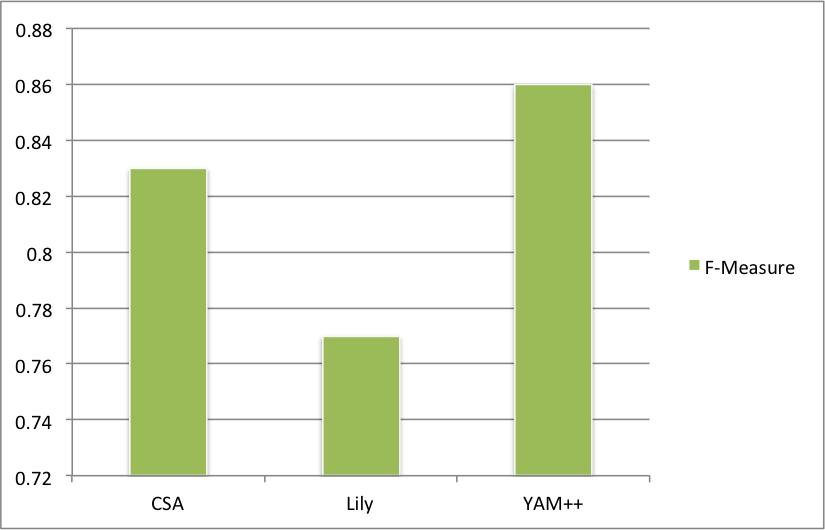
\includegraphics[scale=.5]{figures/oaei/benchmark/top2011.png} 
 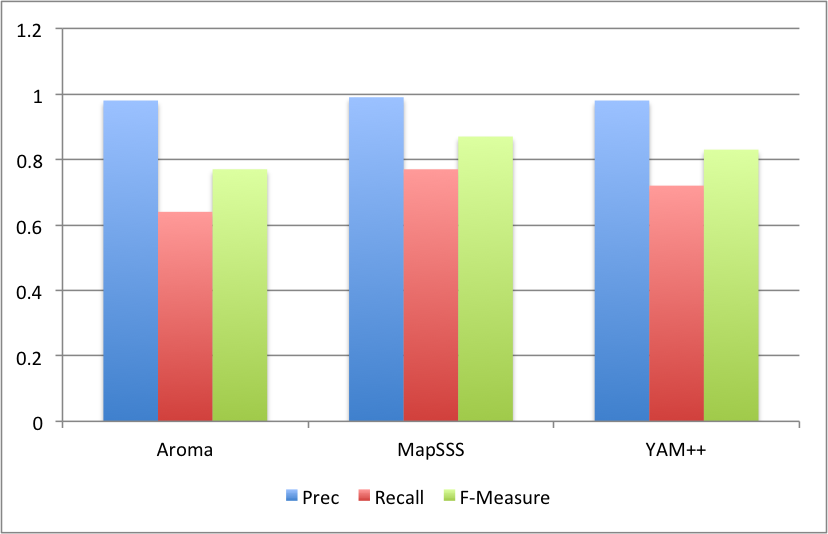
\includegraphics[scale=.5]{figures/oaei/benchmark/top2012.png}
 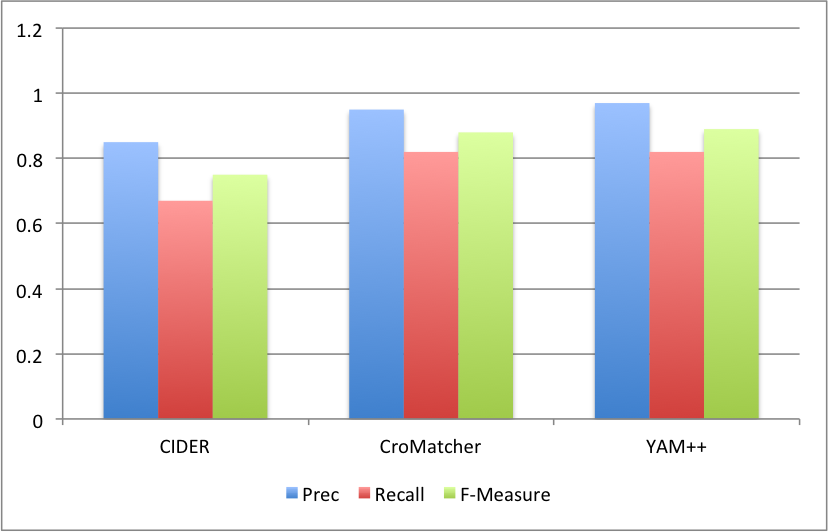
\includegraphics[scale=.5]{figures/oaei/benchmark/top2013.png}  
 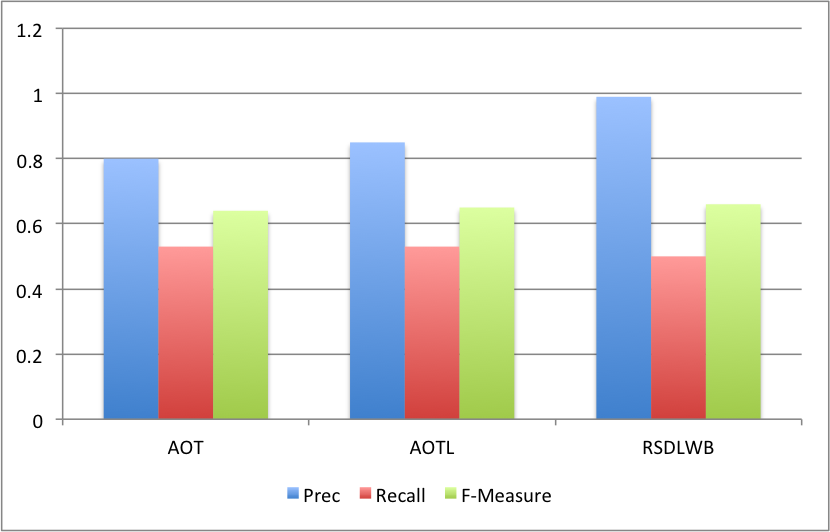
\includegraphics[scale=.5]{figures/oaei/benchmark/top2014.png} 
 \caption{Top performing Ontology Matching Systems for  the OAEI Bibliography Benchmark Dataset}
 \label{img::oaei_anatomy}
\end{figure}

\subsection{Conference}
This data set contains 21 ontologies from the conference domain. They were either created manually, were present or created based on a website of the conference. The ontologies did not change over time and also the alignments between all ontologies are stable. In figure \ref{img::oaei_conf} the result of the top performing matching systems are presented. It can be observed that their has been no real improvement in terms of $f_1-measure$ since 2012. The best systems are AML \cite{Faria:2013aa}, YAM++ \cite{Ngo:2012ab} and LogMap \cite{JimACnez-Ruiz:2011aa}. 

\begin{figure}
 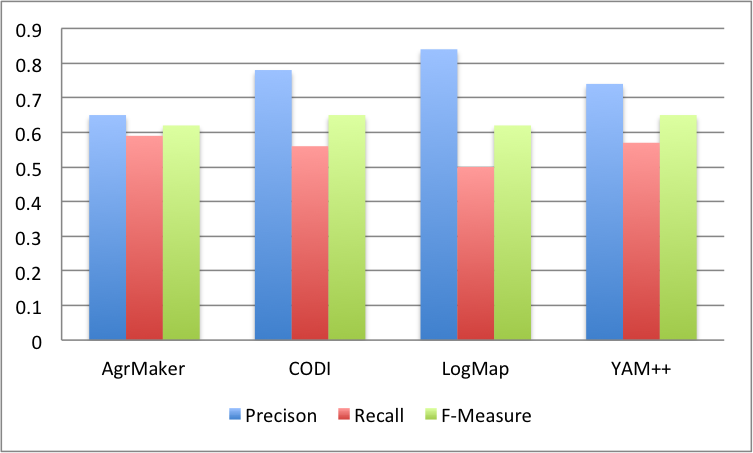
\includegraphics[scale=.5]{figures/oaei/conference/top2011.png} 
 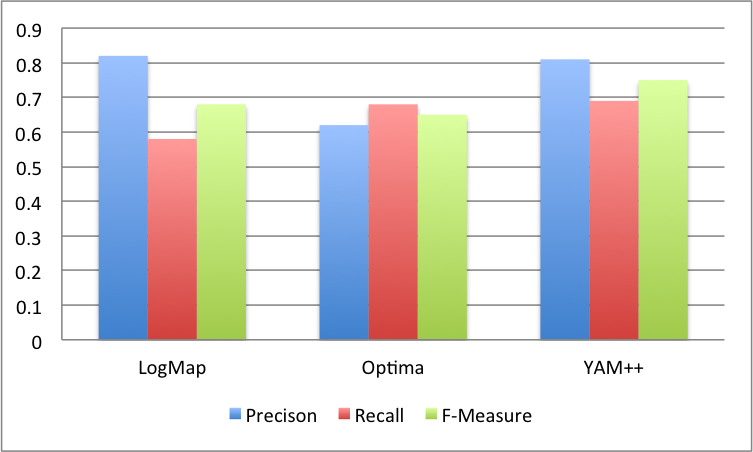
\includegraphics[scale=.5]{figures/oaei/conference/top2012.png}
 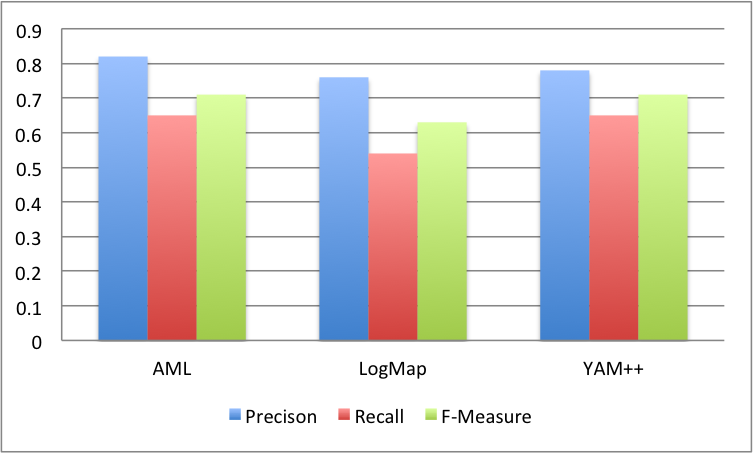
\includegraphics[scale=.5]{figures/oaei/conference/top2013.png}  
 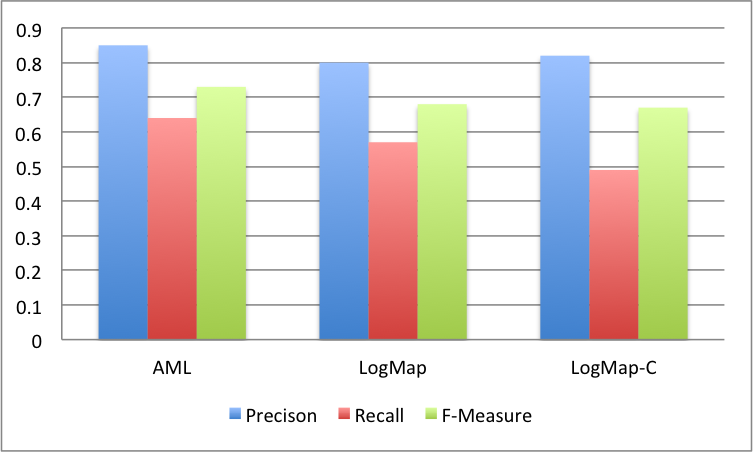
\includegraphics[scale=.5]{figures/oaei/conference/top2014.png} 
 \caption{Top performing Ontology Matching Systems for  the OAEI Conference Dataset}
 \label{img::oaei_conf}
\end{figure}


\subsection{Anatomy}
\label{sec::oaei_anatomy}
For the anatomy dataset the task is set to match the Adult Mouse Anatomy with NCI Thesaurus \footnote{http://ncim.nci.nih.gov/ncimbrowser/}, that describes the human anatomy. The matching task is rather large and results in a big alignment. Despite some changes in the dataset from 2011 to 2012, it was stable over the last two years and therefore comparisons are possible. What can be seen is that there is a clear improvement in terms of $f_1-measure$ over the years, with CODI, AML, GOMMA, YAM++ and LogMap as best performing systems in different periods.

\begin{figure}
 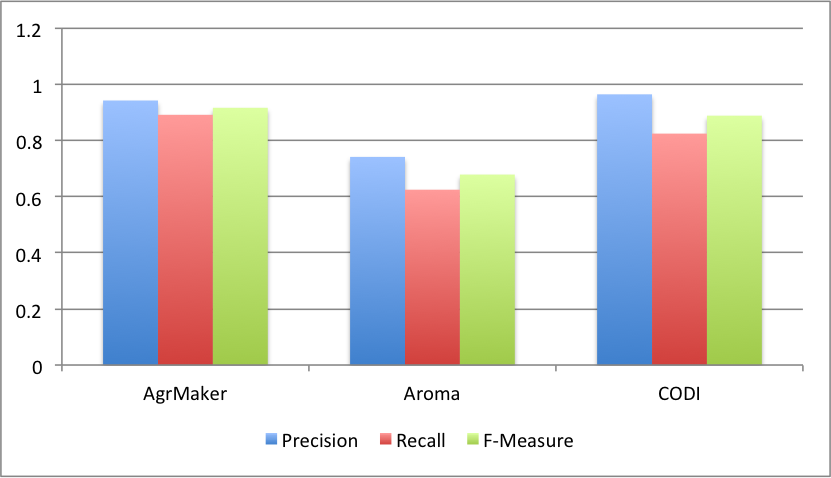
\includegraphics[scale=.5]{figures/oaei/anatomy/top2011.png} 
 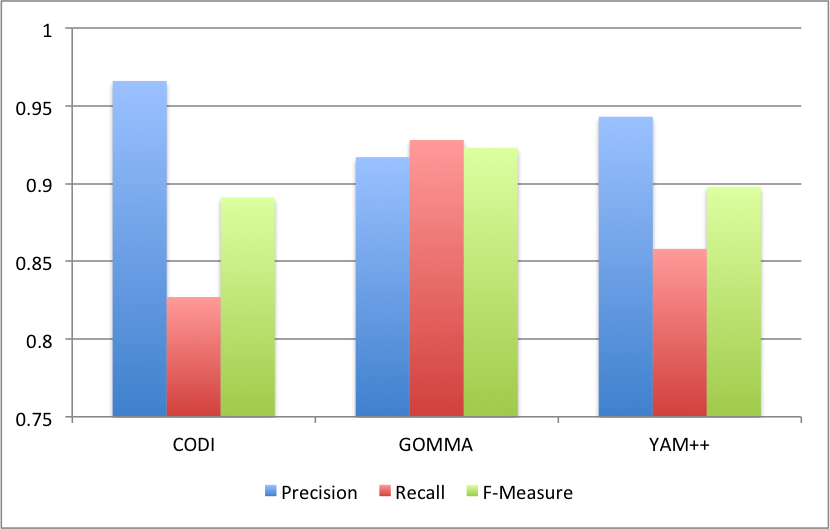
\includegraphics[scale=.5]{figures/oaei/anatomy/top2012.png}
 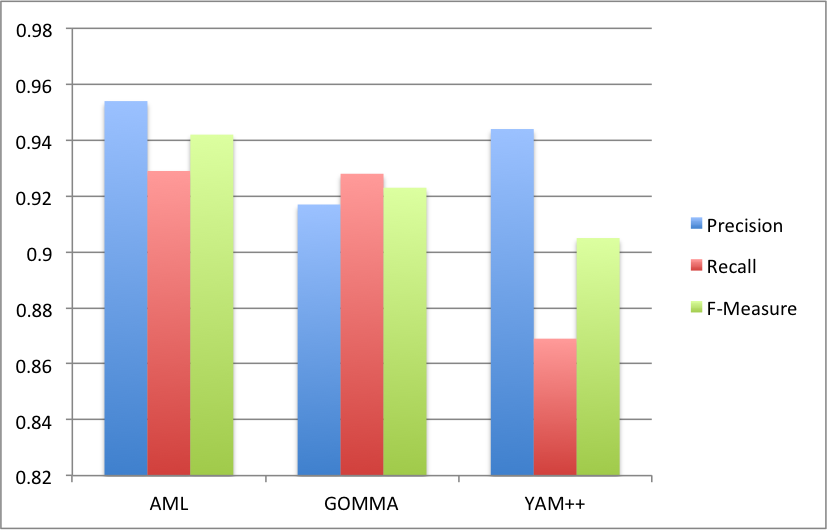
\includegraphics[scale=.5]{figures/oaei/anatomy/top2013.png}  
 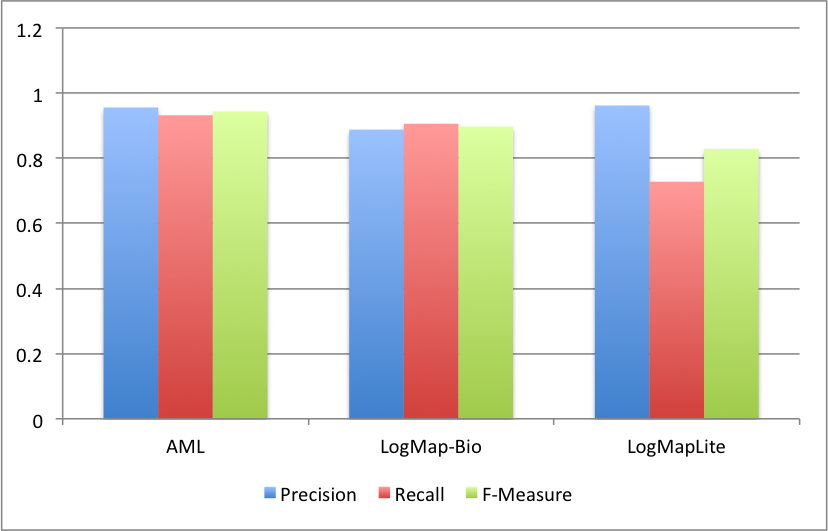
\includegraphics[scale=.5]{figures/oaei/anatomy/top2014.png} 
 \caption{Top performing Ontology Matching Systems for  the OAEI Anatomy Dataset}
 \label{img::oaei_anatomy}
\end{figure}

\subsection{Library}
The OAEI organizers included in 2012 the current 
\begin{figure}
 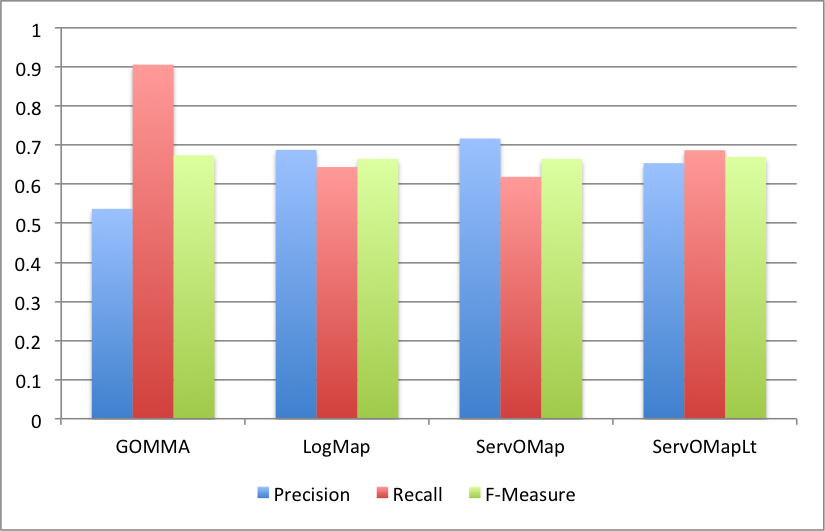
\includegraphics[scale=.5]{figures/oaei/library/top2012.png}
 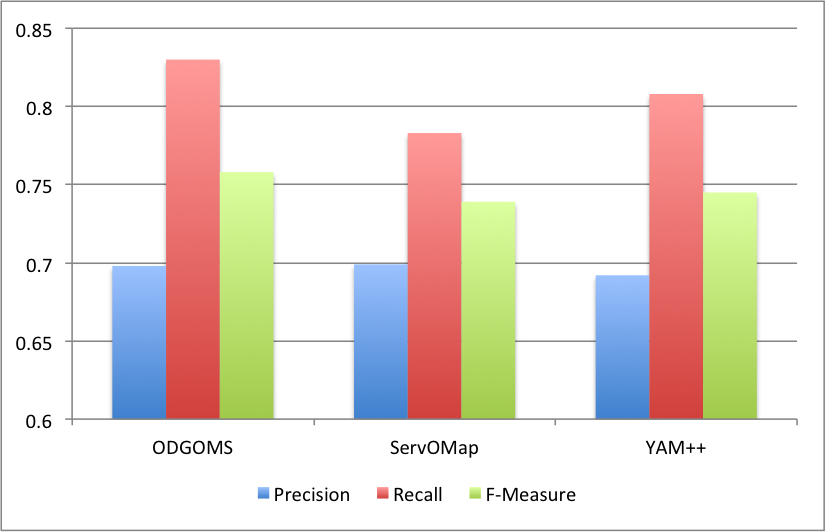
\includegraphics[scale=.5]{figures/oaei/library/top2013.png}  
 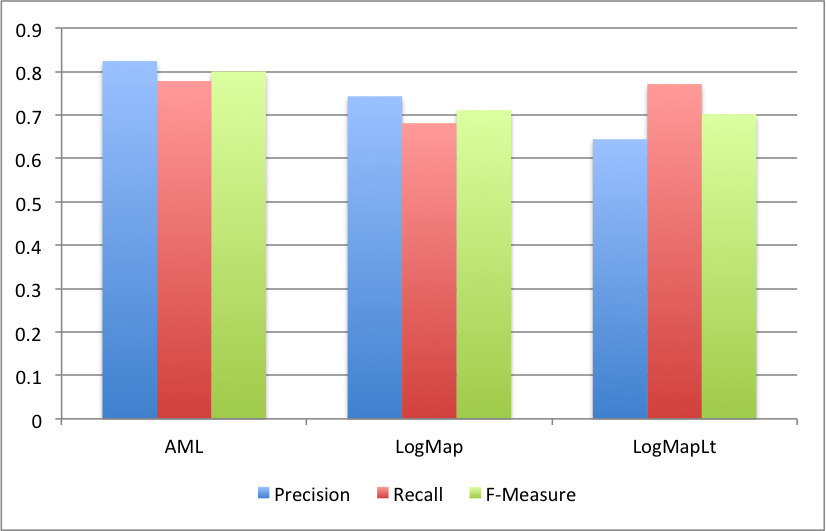
\includegraphics[scale=.5]{figures/oaei/library/top2014.png} 
 \caption{Top performing Ontology Matching Systems for  the OAEI Library Dataset}
 \label{img::library}
\end{figure}

\clearpage
\section{Challenges}
\label{sec:challeng_ontology_matching}
The previous section demonstrated that the ontology matching community is improving their systems in terms of $f_1-measure$. Another way of looking at this is that there still exist various challenges that need be solved, to overcome the disparate dataspace. In \cite{6104044} and  \cite{euzenat2013d} a research agenda with open questions in the field of ontology matching is presented. In addition to that in \cite{OteroCerdeira2015949} a survery was performed among 33 researchers in the field of ontology matching. Table \ref{tab::challenges_in_onto_matching} summarizes the findings.

\begin{table}[h]

\begin{tabular}{c c c}
\hline
Future Challenge &  Shvaiko \& Euzenat & Otero-Cerdeira et. al. \\
\hline
Large Scale and Efficient Matching					& \checked	& \checked           \\                  
Matching with Background Knowledge				& \checked	& \checked    \\                        
Matcher Selection, Combination and Tuning		& \checked	& \checked \\
User Involvement												& \checked	& \checked  \\
Explanation of Matching Results						& \checked	& \checked  \\
Uncertainty in Ontology Matching					& \checked	& \checked  \\
Alignment Management									& \checked	& \checked \\
Improvement of Precision and Recall				&					& \checked \\
Semantic Mapping											&               	& \checked  \\                           
Non-expert user tools										&					& \checked \\
Holistic Ontology Matching								& 					& \checked \\
Complex Relation Detection (non 1:1) 			& 					& \checked \\
Practical Applications of created Mappings		& 					& \checked \\
\hline
\end{tabular}
\caption{Challenges of Ontology Matching Research base on \cite{OteroCerdeira2015949}, \cite{euzenat2013d} and \cite{6104044} }
\label{tab::challenges_in_onto_matching}
\end{table}
However in this thesis the focus lies on the open challenges of \emph{Matcher Selection, Combination and Tuning}. As already mentioned above current matching systems rely on multiple base matchers that have to be combined to create one final 	alignment and try by this to overcome the challenges of heterogenous ontology that need to interoperate. These systems need to elect base matchers and finally combine them  to obtain a comprehensive result. \cite{chuttur2011challenges}

The best way of tackling this problem is to divide into two separate problems, first the matcher selection and second the matcher combination problem.

The first problem can be treated as a feature selection problem, where base matchers are potential useful features that need to be selected. 

On the other hand there is the second problem which describes the combination of the output of the selected base matcher. Current approaches treat this as a weighted average function of the results of the base matchers. This does not incorporate that for matching specific entities some matchers might not be suitable while others predict the correspondence perfectly correct. Therefore there is a need for finding a flexible way to combine the output of selected base matchers, that embraces strength and punishes weakness of individual matchers, aligning judging over a specific correspondence. This leads to the definition of when a flexible ontology matching process.

\begin{definition}[Flexible Ontology  Matching Process]
Inspired by \cite{Ngo:2012aa} in this thesis an ontology matching system is flexible when it automatically selects and combines individual matchers to produce the best possible result in changing data domains.
\end{definition}

To allow a maximum degree of flexibility an unsupervised approach to select and combine multiple matcher will be superior to supervised approaches. Because by this the underlying algorithm does not rely on available training data to match algorithms in a distinct domain. Therefore such an algorithm can used in changing data domains, without additional resources needed. Outlier Detection might a possible methods to perform the combination with the demanded degree of flexibility. 

The best way of summing up this section is to formalize the problem that will be investigated in this master thesis. The goal is to find a meta matching process that selects, runs and combines different individual matching processes, by using a matcher selection function $f_f$ and a combination function $f_c$ in the form of:
\begin{definition}[Meta Ontology Matching Process]
The meta ontology matching process can be seen as a function  of two ontologies $o_1$, $o_2$, a set of individual matching process $F$ (see definition \ref{def::Matching_process}), a combination function $f_c$, a feature selection function $f_f$, a set of parameter $p$ and a set of resource $r$, that return an alignment $A$:

\begin{equation*}
A = f' (o_1,o_1,F, f_c,f_f, p,r)
\end{equation*}
\end{definition}

Of particular interest is to find a selection function $f_f$ that relies on unsupervised methods and a combination function $f_c$ that as well has no need for training. Therefore the use of  outlier analysis as a flexible unsupervised way will be investigated and evaluated in the remainder of this master thesis.

In this section the ontology matching problem in general was introduced and defined, furthermore the current state-of-the art of ontology matching was based on the OAEI presented. Depended on this analysis some challenges from literature for research in ontology matching were enumerated and especially the problem of individual matcher combination and selection was stressed. Finally the meta ontology matching problem was formalized as finding a flexible matching process for blending multiple results into one final alignment, using outlier detection.  Thus in the following section an overview of current individual matching and meta matching techniques is given, in form of an literature review.
%%%%% Bascially Literature review
\chapter{Ontology Matching Approaches (Related Work)}
This chapter presents the results of a conducted literature survey in the area of ontology matching.
\section{Classification of Approaches}
Tailored classification of approaches
\section{Base Matcher}

\subsection{Label Based}
 \subsubsection{TODO}
\subsection{Instance Based}
 \subsubsection{TODO}
\subsection{Structure Based}
 \subsubsection{TODO}
\section{Hybrid Matching Approaches}
\section{Analysis of Hybrid Matching Approaches}
Show weaknesses of current approaches, supervised, often weighted average based, so not flexible (transferable to other domains)

\chapter{Selected Approaches to Outlier Analysis}
\section{Definition Outlier Analysis}
\section{Approaches}

%%%%%%%%%%%%%%%% Main Contribution

\chapter{Hybrid Ontology Matching using Outlier Analysis}
\section{Motivation for using Outlier Analysis for Ontology Matching}
Flexibility towards changing data domains
No need to train weights upfront
\section{Ontology Matching as an Outlier Detection Problem}
\subsection{Creating the Feature Vector}
\subsection{Significance of Outliers for Ontology Matching}
Correlation between Outlier score and label
\subsection{Transforming the Outlier Analysis Result to a Matching}


%%%% Presentation of the Presented Approach
\chapter{A Matching Pipeline using Outlier Detection}

\section{Overview}
Presents the implemented Pipeline
\section{Base Matchers used}
What base matchers survived the selection process
\section{Methods Used to combine Matchers}

\section{Feature Selection}

\section{Outlier Analysis}


%%% Evaluation

\chapter{Evaluation}
\section{Datasets}
\subsection{Conference}
\subsection{Benchmark}
\subsection{Anatomy}
\subsection{Library}
\section{Experimental Setup}
\section{Used Baselines}
\section{Results}


%%% Final Stuff

\chapter{Discussion}
\section{Flexibility towards changing Data Domains}
\section{Runtime Considerations}
\section{Comparison with current OAEI Participants}


\chapter{Conclusion}


% evntuelly you might add something like this
% \listtheorems{definition}
% \listtheorems{proposition}
\clearpage
\newpage


% okay, start new numbering ... here is where it really starts


\bibliographystyle{plain}
\bibliography{bibliography}

\newpage

\pagestyle{empty}


\section*{Ehrenw\"ortliche Erkl\"arung}
Ich versichere, dass ich die beiliegende Bachelorarbeit ohne Hilfe Dritter
und ohne Benutzung anderer als der angegebenen Quellen und Hilfsmittel
angefertigt und die den benutzten Quellen w\"ortlich oder inhaltlich
entnommenen Stellen als solche kenntlich gemacht habe. Diese Arbeit
hat in gleicher oder \"ahnlicher Form noch keiner Pr\"ufungsbeh\"orde
vorgelegen. Ich bin mir bewusst, dass eine falsche Er- kl\"arung rechtliche Folgen haben
wird.
\\
\\

\noindent
Mannheim, den 31.5.2015 \hspace{4cm} Unterschrift

\end{document}
